\documentclass[12pt]{article}
\usepackage[spanish]{babel}

%%%%%%%%%%%%%%%%%%%%%%%%%%%%%%%%%%
%%%%%%%%%%%%%%%%%%%%%%%%%%%%%   %%
%%        Datos Trabajo     %%  %%
%%%%%%%%%%%%%%%%%%%%%%%%%%%%%%%%%%
\newcommand{\titulo}[0]{ Actividad 3. Representación de datos estadísticos por medio de graficas}
\newcommand{\materia}[0]{Estad\'istica B\'asica}
\newcommand{\grupo}[0]{BI-BEBA-2002-B2-013}
\newcommand{\unidad}[0]{Unidad 2}


%%%%%%%%%%%%%%%%%%%%%%%%%%%%%%%%%%
%%%%%%%%%%%%%%%%%%%%%%%%%%%%%%%%%%
\usepackage{amssymb}
\usepackage{enumerate}
\usepackage{geometry}
\usepackage{mathtools}
\usepackage{multicol}
\usepackage{soul}

\usepackage{graphicx}
	\graphicspath{ {assets/} }

\usepackage{hyperref}
	\hypersetup{
			pdftex,
		        pdfauthor={bench},
		        pdftitle={\titulo},
		        pdfsubject={\materia},
		        pdfkeywords={\grupo, \unidad, UnADM},
		        pdfproducer={Latex with hyperref, Ubuntu},
		        pdfcreator={pdflatex, or other tool},
			colorlinks=true,
				linkcolor=red,
				urlcolor=cyan,
				filecolor=green,
				citecolor=blue}

%%%%%%%%%%%%%%%%%%%%%%%%%%%%%%%%%%
%%%%%%%%%%%%%%%%%%%%%%%%%%%%%%%%%%

\title{
	
\includegraphics{../../../assets/logo-unadm} \\
	\ \\ Benjam\'in Rivera \\
	\bf{\titulo}\\\ \\}

\author{
	Universidad Abierta y a Distancia de México \\
	TSU en Biotecnolog\'ia \\
	\textit{Materia:} \materia \\
	\textit{Grupo:} \grupo \\
	\textit{Unidad:} \unidad \\
	\\
	\textit{Matricula:} ES202105994 }

\date{\textit{Fecha de entrega:} \today}


%%%%%%%%%%%%%%%%%%%%%%%%%%%%%
%%        Documento         %%
%%%%%%%%%%%%%%%%%%%%%%%%%%%%%%%
\begin{document}
\maketitle\newpage

	\par Primero volveremos a poner la tabla inicial para recordar los datos con los que estamos trabajando. Estos datos, y sus distribuciones, se pueden apreciar en la figura~\ref{fig: tabla}.
	
	\begin{figure}[htp]
		\centering
			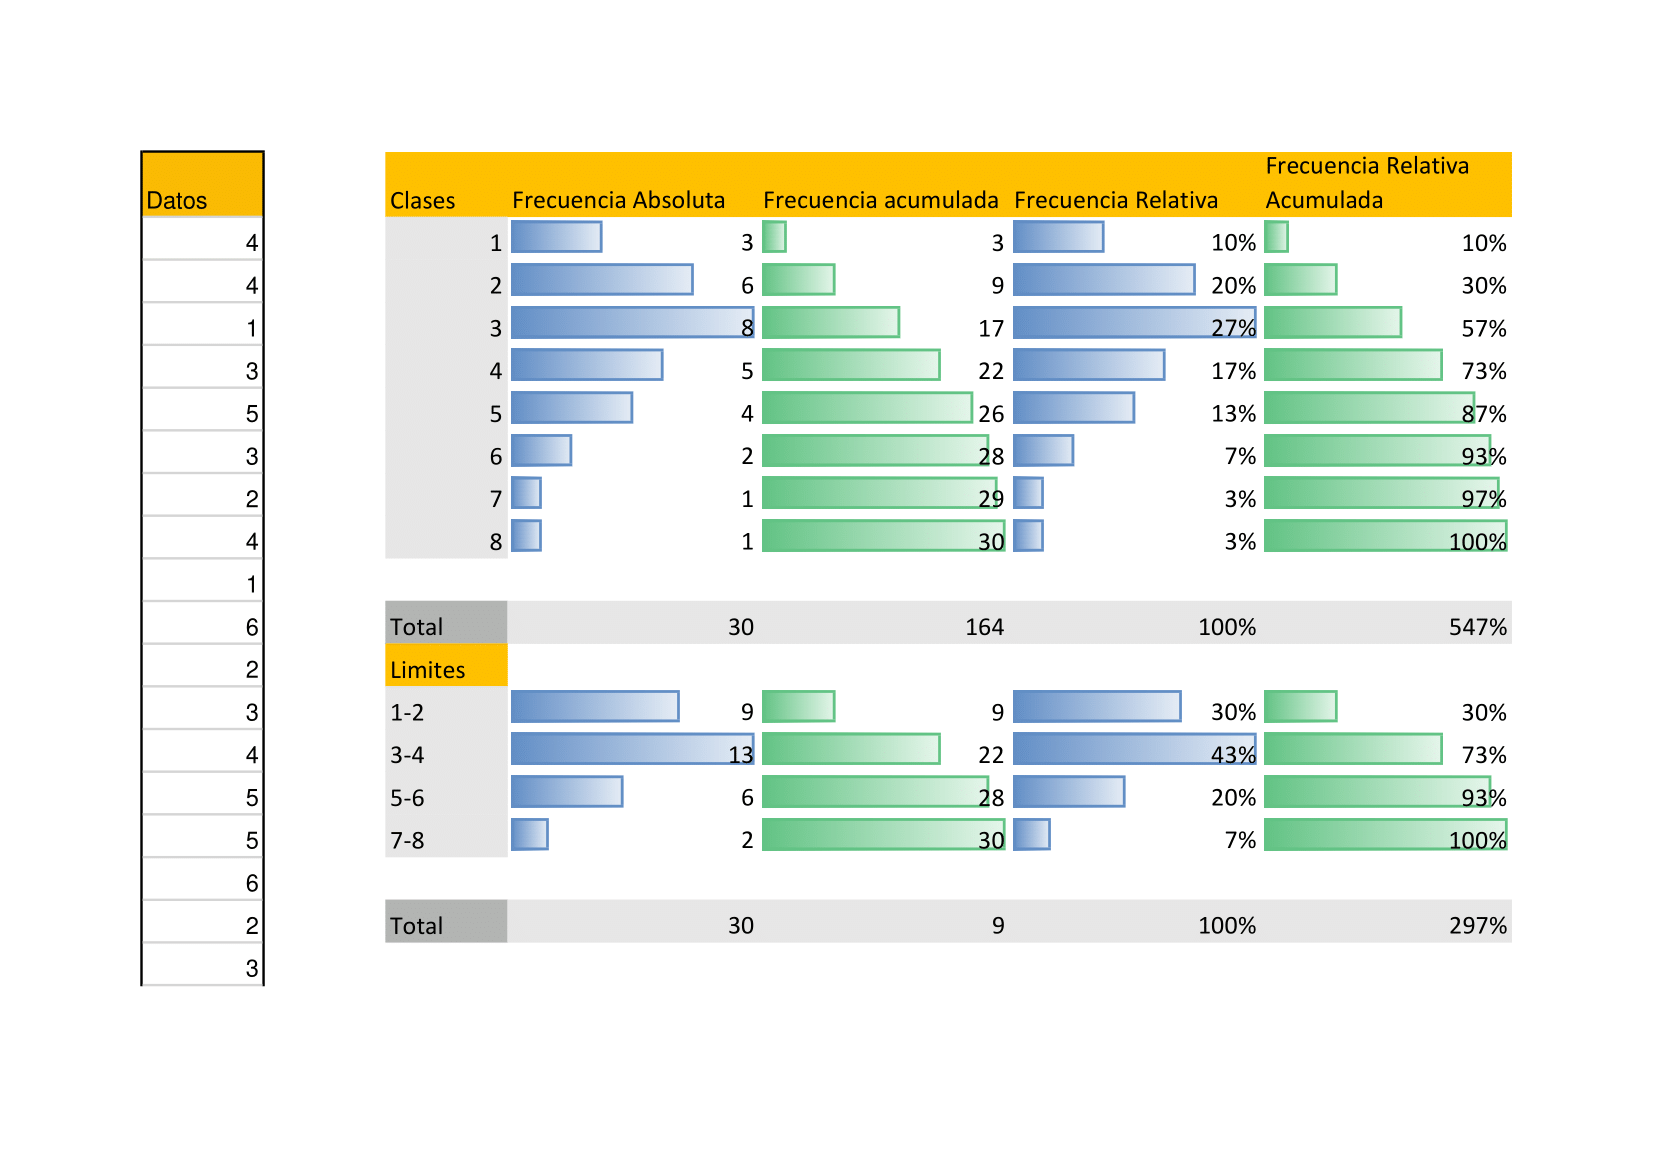
\includegraphics[width=0.9\textwidth]{Book1.png}
		\caption{Tabla de distribuci\'on de frecuencias de los datos de la actividad anterior.}
		\label{fig: tabla}
	\end{figure}
	
	\par Ahora que recordamos los datos, lo primero que me gustar\'ia poder comprender mejor es la manera global en que se distribuyen las frecuencias con las clases. Para esto me parece ideal el gr\'afico de pastel, que implementado lo podemos ver en la figura~\ref{fig: gr 1}; esta elecci\'on me parece la mejor porque nos permite apreciar, en una sola mirada, en comparaci\'on del universo con el que estemos trabajando, todos los elementos de nuestras clases.
	
	\par El principal inconveniente de la representaci\'on anterior la veo en que los datos individuales son difíciles de leer, adem\'as de que una distribuci\'on estad\'istica no es tan f\'acil de observar en esta represetaci\'on. Para mejorar esto est\'an los histogramas, que presentan los datos de una manera m\'as accesibles. Creo que con nuestros datos esto se nota m\'as cuando graficamos las clases contra las frecuencias absolutas, esto se puede apreciar en la figura~\ref{fig: gr 2}.

	\begin{figure}[htp]
		\centering
			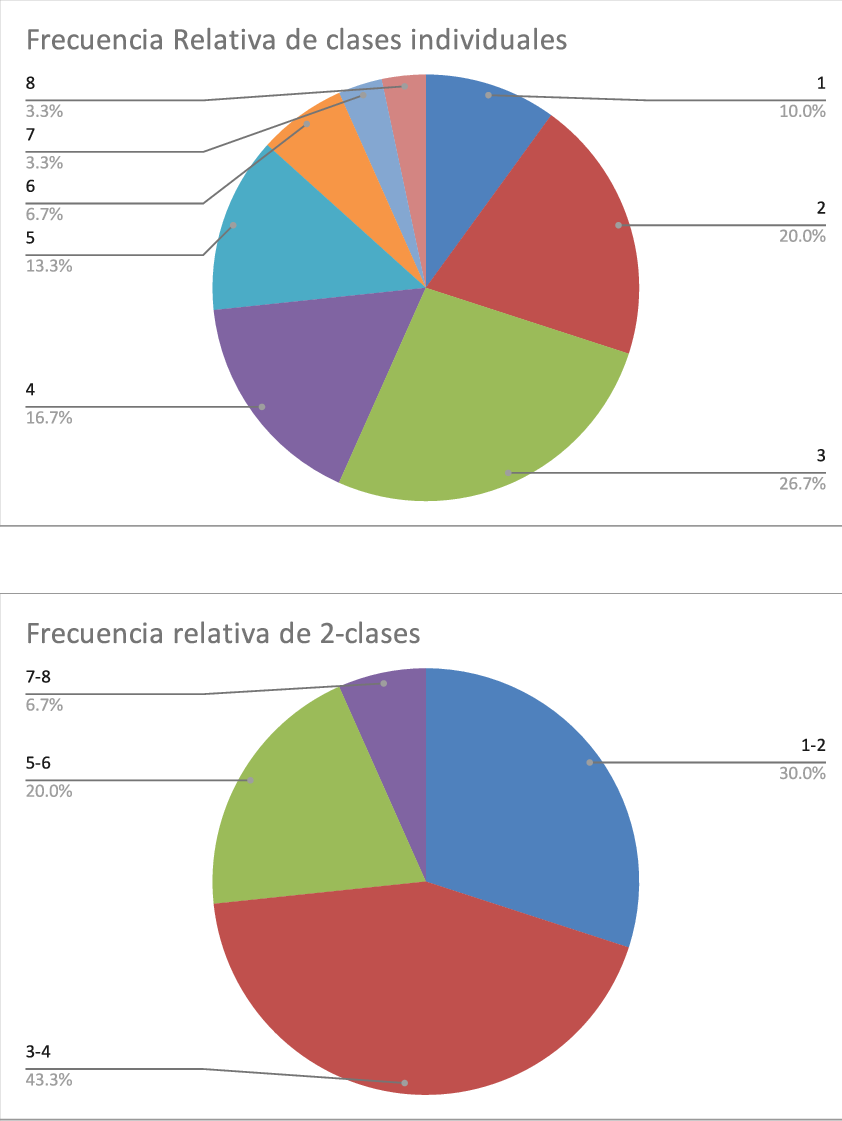
\includegraphics[width=0.8\textwidth]{Graficas-0.png}
		\caption{Gráficos circulares de la distribuci\'on de frecuencias relativas.}
		\label{fig: gr 1}
	\end{figure}
	\begin{figure}[htp]
		\centering
			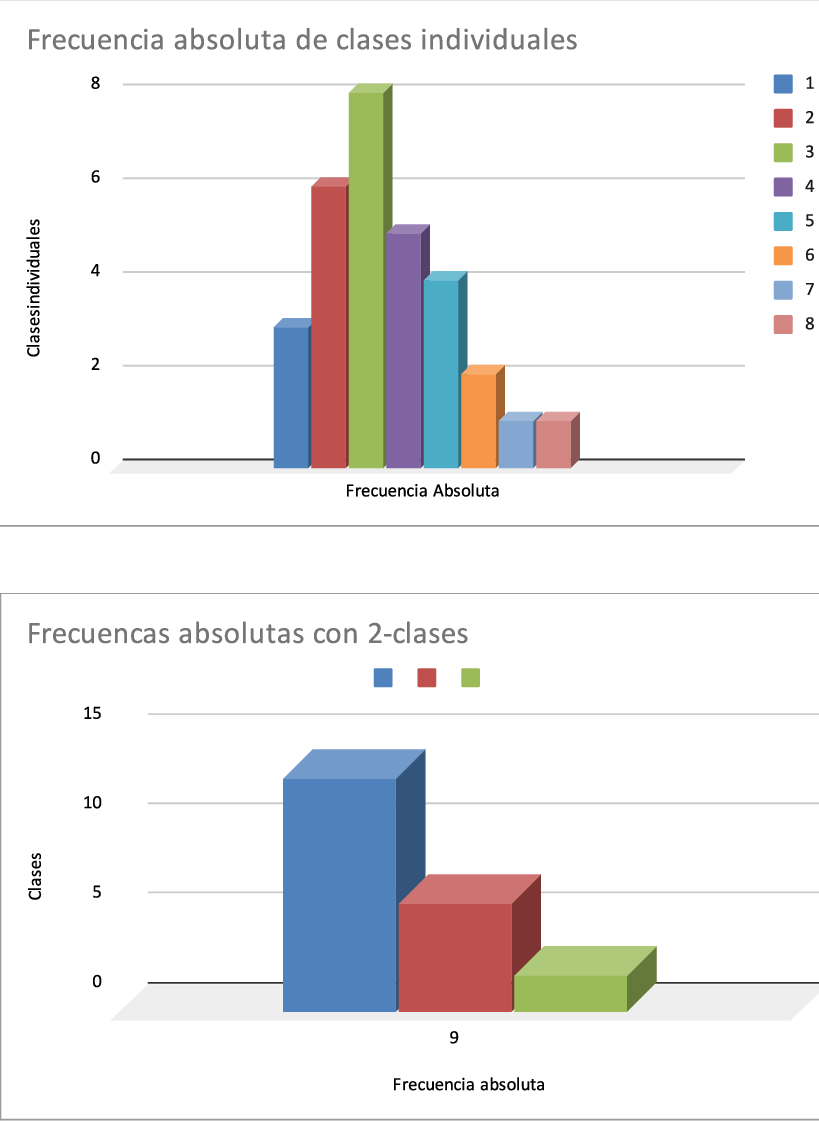
\includegraphics[width=0.8\textwidth]{Graficas-1.png}
		\caption{Histograma de las frecuencias absolutas.}
		\label{fig: gr 2}
	\end{figure}



%%%%%%%%%%%%%%%%%%%%%%%%%%%%%%%%
%%         Bibliografia        %%
%%%%%%%%%%%%%%%%%%%%%%%%%%%%%%%%%%
\newpage
\begin{thebibliography}{X}
	\bibitem{biblio1} Borrego del Pino, S. (2018). \textit{ESTADÍSTICA DESCRIPTIVA E INFERENCIAL}. csif. \url{https://archivos.csif.es/archivos/andalucia/ensenanza/revistas/csicsif/revista/pdf/Numero_13/SILVIA_BORREGO_2.pdf}
	\bibitem{biblio2} Espinel F., C. (s. f.). LAS GRÁFICAS ESTAD\'ISTICAS. Research Gate. \url{https://www.researchgate.net/profile/Maria_Teresa_Gonzalez2/publication/295699313_LAS_GRAFICAS_ESTADISTICAS/links/56cc89d308ae1106370d9912/LAS-GRAFICAS-ESTADISTICAS.pdf}
	\bibitem{biblio3} Gráficas estadísticas $|$ Matemáticas. (s/f). bartolomecossio. Recuperado el 17 de octubre de 2020, de \url{http://www.bartolomecossio.com/MATEMATICAS/grficas_estadsticas.html}

\end{thebibliography}

\end{document}